%\documentclass{article}
%\usepackage{beamerarticle}
\documentclass[serif,ignorenonframetext]{beamer}

% Macros for MATH 110 course dates

\newcommand{\commonTheme}{metropolis}
\newcommand{\commonColorTheme}{metropolis}

\newcommand{\commonAuthor}{Edward Doolittle}
\newcommand{\commonInstitute}{Department of Indigenous Knowledge and
  Science \\ First Nations University of Canada}
\newcommand{\commonCourse}{MATH 110 Calculus I}
\newcommand{\commonTerm}{202510}
\newcommand{\commonDate}{January 6, 2025}

% Review Material

% Lab 0
\newcommand{\commonEventNegativeOne}{LabNegativeOne}
\newcommand{\commonDateLabNegativeOne}{Monday, January 6, 2025}
\newcommand{\commonTitleLabNegativeOne}{MATH 110 Lab 0}
\newcommand{\commonSubtitleLabNegativeOne}{No Lab; Course Opens}

% Section 001
\newcommand{\commonEventZeroZeroOne}{ZeroZeroOne}
\newcommand{\commonDateZeroZeroOne}{Tuesday, January 7, 2025}
\newcommand{\commonTitleZeroZeroOne}{MATH 110 Review 0.1}
\newcommand{\commonSubtitleZeroZeroOne}{Review of Algebra}
\newcommand{\commonPSTitleZeroZeroOne}{MATH 110 Review Problem Set 0.1}

% Section 00A
\newcommand{\commonEventZeroZeroA}{ZeroZeroA}
\newcommand{\commonDateZeroZeroA}{Tuesday, January 7, 2025}
\newcommand{\commonTitleZeroZeroA}{MATH 110 Review 0.A}
\newcommand{\commonSubtitleZeroZeroA}{Review of Inequalities and
  Absolute Values}
\newcommand{\commonPSTitleZeroZeroA}{MATH 110 Review Problem Set 0.A}

% Section 00B
\newcommand{\commonEventZeroZeroB}{ZeroZeroB}
\newcommand{\commonDateZeroZeroB}{Tuesday, January 7, 2025}
\newcommand{\commonTitleZeroZeroB}{MATH 110 Review 0.B}
\newcommand{\commonSubtitleZeroZeroB}{Review of Coordinate Geometry
  and Lines}
\newcommand{\commonPSTitleZeroZeroB}{MATH 110 Review Problem Set 0.B}

% Section 00C
\newcommand{\commonEventZeroZeroC}{ZeroZeroC}
\newcommand{\commonDateZeroZeroC}{Thursday, January 9, 2025}
\newcommand{\commonTitleZeroZeroC}{MATH 110 Review 0.C}
\newcommand{\commonSubtitleZeroZeroC}{Review of Graphs of Second
  Degree Equations}
\newcommand{\commonPSTitleZeroZeroC}{MATH 110 Review Problem Set 0.C}

% Section 00D
\newcommand{\commonEventZeroZeroD}{ZeroZeroD}
\newcommand{\commonDateZeroZeroD}{Thursday, January 9, 2025}
\newcommand{\commonTitleZeroZeroD}{MATH 110 Review 0.D}
\newcommand{\commonSubtitleZeroZeroD}{Review of Trigonometry}
\newcommand{\commonPSTitleZeroZeroD}{MATH 110 Review Problem Set 0.D}

% Section 011
\newcommand{\commonEventZeroOneOne}{ZeroOneOne}
\newcommand{\commonDateZeroOneOne}{Thursday, January 9, 2025}
\newcommand{\commonTitleZeroOneOne}{MATH 110 Review 1.1}
\newcommand{\commonSubtitleZeroOneOne}{Review of Functions}
\newcommand{\commonPSTitleZeroOneOne}{MATH 110 Review Problem Set 1.1}


% Main Course

% Lab 1
\newcommand{\commonEventZero}{LabZero}
\newcommand{\commonDateLabZero}{Monday, January 13, 2025}
\newcommand{\commonTitleLabZero}{MATH 110 Lab 1}
\newcommand{\commonSubtitleLabZero}{Quiz 0: STACK, Onboarding}

% Section 1.4
\newcommand{\commonEventOne}{ZeroOneFour}
\newcommand{\commonDateZeroOneFour}{Tuesday, January 14, 2025}
\newcommand{\commonTitleZeroOneFour}{MATH 110 Lecture 1.4}
\newcommand{\commonSubtitleZeroOneFour}{The Tangent and Velocity Problems}
\newcommand{\commonPSTitleZeroOneFour}{MATH 110 Problem Set 1.4}

% Section 1.5
\newcommand{\commonEventTwo}{ZeroOneFive}
\newcommand{\commonDateZeroOneFive}{Thursday, January 16, 2025}
\newcommand{\commonTitleZeroOneFive}{MATH 110 Lecture 1.5}
\newcommand{\commonSubtitleZeroOneFive}{The Limit of a Function}
\newcommand{\commonPSTitleZeroOneFive}{MATH 110 Problem Set 1.5}

% Lab 2
\newcommand{\commonEventThree}{LabOne}
\newcommand{\commonDateLabOne}{Monday, January 20, 2025}
\newcommand{\commonTitleLabOne}{MATH 110 Lab 2}
\newcommand{\commonSubtitleLabOne}{Quiz 1: Review}

% Section 1.6
\newcommand{\commonEventFour}{ZeroOneSix}
\newcommand{\commonDateZeroOneSix}{Tuesday, January 21, 2025}
\newcommand{\commonTitleZeroOneSix}{MATH 110 Lecture 1.6}
\newcommand{\commonSubtitleZeroOneSix}{Calculating Limits Using the Limit Laws}
\newcommand{\commonPSTitleZeroOneSix}{MATH 110 Problem Set 1.6}

% Section 1.7
\newcommand{\commonEventFive}{ZeroOneSeven}
\newcommand{\commonDateZeroOneSeven}{(Not covered)}
\newcommand{\commonTitleZeroOneSeven}{MATH 110 Lecture 1.7}
\newcommand{\commonSubtitleZeroOneSeven}{The Precise Definition of a Limit}
\newcommand{\commonPSTitleZeroOneSeven}{MATH 110 Problem Set 1.7}

% Section 1.8
\newcommand{\commonEventSix}{ZeroOneEight}
\newcommand{\commonDateZeroOneEight}{Thursday, January 23, 2025}
\newcommand{\commonTitleZeroOneEight}{MATH 110 Lecture 1.8}
\newcommand{\commonSubtitleZeroOneEight}{Continuity}
\newcommand{\commonPSTitleZeroOneEight}{MATH 110 Problem Set 1.8}

% Lab 3
\newcommand{\commonEventSeven}{LabTwo}
\newcommand{\commonDateLabTwo}{Monday, January 27, 2025}
\newcommand{\commonTitleLabTwo}{MATH 110 Lab 3}
\newcommand{\commonSubtitleLabTwo}{Quiz 2: Sections 1.4, 1.5}

% Section 2.1
\newcommand{\commonEventEight}{ZeroTwoOne}
\newcommand{\commonDateZeroTwoOne}{Tuesday, January 28, 2025}
\newcommand{\commonTitleZeroTwoOne}{MATH 110 Lecture 2.1}
\newcommand{\commonSubtitleZeroTwoOne}{Derivatives and Rates of Change}
\newcommand{\commonPSTitleZeroTwoOne}{MATH 110 Problem Set 2.1}

% Section 2.2
\newcommand{\commonEventNine}{ZeroTwoTwo}
\newcommand{\commonDateZeroTwoTwo}{Thursday, January 30, 2025}
\newcommand{\commonTitleZeroTwoTwo}{MATH 110 Lecture 2.2}
\newcommand{\commonSubtitleZeroTwoTwo}{The Derivative as a Function}
\newcommand{\commonPSTitleZeroTwoTwo}{MATH 110 Problem Set 2.2}

% Lab 4
\newcommand{\commonEventTen}{LabThree}
\newcommand{\commonDateMTOne}{Monday, February 3, 2025} 
\newcommand{\commonDateLabThree}{Monday, February 3, 2025}
\newcommand{\commonTitleLabThree}{MATH 110 Lab 4}
\newcommand{\commonSubtitleLabThree}{Midterm: Review, Chapter 1}

% Section 2.3
\newcommand{\commonEventEleven}{ZeroTwoThree}
\newcommand{\commonDateZeroTwoThree}{Tuesday, February 4, 2025}
\newcommand{\commonTitleZeroTwoThree}{MATH 110 Lecture 2.3}
\newcommand{\commonSubtitleZeroTwoThree}{Differentiation Formulas}
\newcommand{\commonPSTitleZeroTwoThree}{MATH 110 Problem Set 2.3}

% Section 2.4
\newcommand{\commonEventTwelve}{ZeroTwoFour}
\newcommand{\commonDateZeroTwoFour}{Thursday, February 6, 2025}
\newcommand{\commonTitleZeroTwoFour}{MATH 110 Lecture 2.4}
\newcommand{\commonSubtitleZeroTwoFour}{Derivatives of Trigonometric Functions}
\newcommand{\commonPSTitleZeroTwoFour}{MATH 110 Problem Set 2.4}

% Lab 5
\newcommand{\commonEventThirteen}{LabFour}
\newcommand{\commonDateLabFour}{Monday, February 10, 2025}
\newcommand{\commonTitleLabFour}{MATH 110 Lab 5}
\newcommand{\commonSubtitleLabFour}{Quiz 3: Sections 2.1, 2.2}

% Section 2.5
\newcommand{\commonEventFourteen}{ZeroTwoFive}
\newcommand{\commonDateZeroTwoFive}{Tuesday, February 11, 2025}
\newcommand{\commonTitleZeroTwoFive}{MATH 110 Lecture 2.5}
\newcommand{\commonSubtitleZeroTwoFive}{The Chain Rule}
\newcommand{\commonPSTitleZeroTwoFive}{MATH 110 Problem Set 2.5}

% Section 2.6
\newcommand{\commonEventFifteen}{ZeroTwoSix}
\newcommand{\commonDateZeroTwoSix}{Thursday, February 13, 2025}
\newcommand{\commonTitleZeroTwoSix}{MATH 110 Lecture 2.6}
\newcommand{\commonSubtitleZeroTwoSix}{Implicit Differentiation}
\newcommand{\commonPSTitleZeroTwoSix}{MATH 110 Problem Set 2.6}

% Lab 6
\newcommand{\commonEventSixteen}{LabFive}
\newcommand{\commonDateLabFive}{Monday, February 24, 2025}
\newcommand{\commonTitleLabFive}{MATH 110 Lab 6}
\newcommand{\commonSubtitleLabFive}{Quiz 4: Sections 2.3, 2.4}

% Section 2.7
\newcommand{\commonEventSeventeen}{ZeroTwoSeven}
\newcommand{\commonDateZeroTwoSeven}{Tuesday, February 25, 2025}
\newcommand{\commonTitleZeroTwoSeven}{MATH 110 Lecture 2.7}
\newcommand{\commonSubtitleZeroTwoSeven}{Rates of Change in the
  Natural and Social Sciences}
\newcommand{\commonPSTitleZeroTwoSeven}{MATH 110 Problem Set 2.7}

% Section 2.8
\newcommand{\commonEventEighteen}{ZeroTwoEight}
\newcommand{\commonDateZeroTwoEight}{Thursday, February 27, 2025}
\newcommand{\commonTitleZeroTwoEight}{MATH 110 Lecture 2.8}
\newcommand{\commonSubtitleZeroTwoEight}{Related Rates}
\newcommand{\commonPSTitleZeroTwoEight}{MATH 110 Problem Set 2.8}

% Lab 7
\newcommand{\commonEventNineteen}{LabSix}
\newcommand{\commonDateLabSix}{Monday, March 3, 2025}
\newcommand{\commonTitleLabSix}{MATH 110 Lab 7}
\newcommand{\commonSubtitleLabSix}{Quiz 5: Sections 2.5, 2.6}

% Section 3.1
\newcommand{\commonEventTwenty}{ZeroThreeOne}
\newcommand{\commonDateZeroThreeOne}{Tuesday, March 4, 2025}
\newcommand{\commonTitleZeroThreeOne}{MATH 110 Lecture 3.1}
\newcommand{\commonSubtitleZeroThreeOne}{Maximum and Minimum Values}
\newcommand{\commonPSTitleZeroThreeOne}{MATH 11 Problem Set 3.1}

% Section 3.2
\newcommand{\commonEventTwentyOne}{ZeroThreeTwo}
\newcommand{\commonDateZeroThreeTwo}{Thursday, March 6, 2025}
\newcommand{\commonTitleZeroThreeTwo}{MATH 110 Lecture 3.2}
\newcommand{\commonSubtitleZeroThreeTwo}{The Mean Value Theorem}
\newcommand{\commonPSTitleZeroThreeTwo}{MATH 110 Problem Set 3.2}

% Lab 8
\newcommand{\commonEventTwentyTwo}{LabSeven}
\newcommand{\commonDateMTTwo}{Monday, March 10, 2025}
\newcommand{\commonDateLabSeven}{Monday, March 10, 2025}
\newcommand{\commonTitleLabSeven}{MATH 110 Lab 8}
\newcommand{\commonSubtitleLabSeven}{Midterm: Chapter 2}

% Section 3.3
\newcommand{\commonEventTwentyThree}{ZeroThreeThree}
\newcommand{\commonDateZeroThreeThree}{Tuesday, March 11, 2025}
\newcommand{\commonTitleZeroThreeThree}{MATH 110 Lecture 3.3}
\newcommand{\commonSubtitleZeroThreeThree}{How Derivatives Affect the
  Shape of a Graph}
\newcommand{\commonPSTitleZeroThreeThree}{MATH 110 Problem Set 3.3}

% Section 3.4
\newcommand{\commonEventTwentyFour}{ZeroThreeFour}
\newcommand{\commonDateZeroThreeFour}{Thursday, March 13, 2025}
\newcommand{\commonTitleZeroThreeFour}{MATH 110 Lecture 3.4}
\newcommand{\commonSubtitleZeroThreeFour}{Limits at Infinity;
  Horizontal Asymptotes}
\newcommand{\commonPSTitleZeroThreeFour}{MATH 110 Problem Set 3.4}

% Lab 9
\newcommand{\commonEventTwentyFive}{LabEight}
\newcommand{\commonDateLabEight}{Monday, March 17, 2025}
\newcommand{\commonTitleLabEight}{MATH 110 Lab 9}
\newcommand{\commonSubtitleLabEight}{Quiz 6: Sections 3.1, 3.2}

% Section 3.5
\newcommand{\commonEventTwentySix}{ZeroThreeFive}
\newcommand{\commonDateZeroThreeFive}{Tuesday, March 18, 2025}
\newcommand{\commonTitleZeroThreeFive}{MATH 110 Lecture 3.5}
\newcommand{\commonSubtitleZeroThreeFive}{Summary of Curve Sketching}
\newcommand{\commonPSTitleZeroThreeFive}{MATH 110 Problem Set 3.5}

% Section 3.7
\newcommand{\commonEventTwentySeven}{ZeroThreeSeven}
\newcommand{\commonDateZeroThreeSeven}{Thursday, March 20, 2025}
\newcommand{\commonTitleZeroThreeSeven}{MATH 110 Lecture 3.7}
\newcommand{\commonSubtitleZeroThreeSeven}{Optimization Problems}
\newcommand{\commonPSTitleZeroThreeSeven}{MATH 110 Problem Set 3.7}

% Lab 10
\newcommand{\commonEventTwentyEight}{LabNine}
\newcommand{\commonDateLabNine}{Monday, March 24, 2025}
\newcommand{\commonTitleLabNine}{MATH 110 Lab 10}
\newcommand{\commonSubtitleLabNine}{Quiz 7: Sections 3.3, 3.4}

% Section 4.1
\newcommand{\commonEventTwentyNine}{ZeroFourOne}
\newcommand{\commonDateZeroFourOne}{Tuesday, March 25, 2025}
\newcommand{\commonTitleZeroFourOne}{MATH 110 Lecture 4.1}
\newcommand{\commonSubtitleZeroFourOne}{Areas and Distances}
\newcommand{\commonPSTitleZeroFourOne}{MATH 110 Problem Set 4.1}

% Section 4.2
\newcommand{\commonEventThirty}{ZeroFourTwo}
\newcommand{\commonDateZeroFourTwo}{Thursday, March 27, 2025}
\newcommand{\commonTitleZeroFourTwo}{MATH 110 Lecture 4.2}
\newcommand{\commonSubtitleZeroFourTwo}{The Definite Integral}
\newcommand{\commonPSTitleZeroFourTwo}{MATH 110 Problem Set 4.2}

% Lab 11
\newcommand{\commonEventThirtyOne}{LabTen}
\newcommand{\commonDateLabTen}{Monday, March 31, 2025}
\newcommand{\commonTitleLabTen}{MATH 110 Lab 11}
\newcommand{\commonSubtitleLabTen}{Quiz 8: Sections 3.5, 3.7}

% Section 4.3
\newcommand{\commonEventThirtyTwo}{ZeroFourThree}
\newcommand{\commonDateZeroFourThree}{Tuesday, April 1, 2025}
\newcommand{\commonTitleZeroFourThree}{MATH 110 Lecture 4.3}
\newcommand{\commonSubtitleZeroFourThree}{The Fundamental Theorem of Calculus}
\newcommand{\commonPSTitleZeroFourThree}{MATH 110 Problem Set 4.3}

% Section 4.4
\newcommand{\commonEventThirtyThree}{ZeroFourFour}
\newcommand{\commonDateZeroFourFour}{Thursday, April 3, 2025}
\newcommand{\commonTitleZeroFourFour}{MATH 110 Lecture 4.4}
\newcommand{\commonSubtitleZeroFourFour}{Indefinite Integrals and the
  Net Change Theorem}
\newcommand{\commonPSTitleZeroFourFour}{MATH 110 Problem Set 4.4}

% Lab 12
\newcommand{\commonEventThirtyFour}{LabEleven}
\newcommand{\commonDateLabEleven}{Monday, April 7, 2025}
\newcommand{\commonTitleLabEleven}{MATH 110 Lab 12}
\newcommand{\commonSubtitleLabEleven}{Quiz 9: Sections 4.1, 4.2}

% Section 4.5
\newcommand{\commonEventThirtyFive}{ZeroFourFive}
\newcommand{\commonDateZeroFourFive}{Tuesday, April 8, 2025}
\newcommand{\commonTitleZeroFourFive}{MATH 110 Lecture 4.5}
\newcommand{\commonSubtitleZeroFourFive}{The Substitution Rule}
\newcommand{\commonPSTitleZeroFourFive}{MATH 110 Problem Set 4.5}

% Section 5.1
\newcommand{\commonEventThirtySix}{ZeroFiveOne}
\newcommand{\commonDateZeroFiveOne}{Thursday, April 10, 2025}
\newcommand{\commonTitleZeroFiveOne}{MATH 110 Lecture 5.1}
\newcommand{\commonSubtitleZeroFiveOne}{Areas Between Curves}
\newcommand{\commonPSTitleZeroFiveOne}{MATH 110 Problem Set 5.1}

% Lab 13
\newcommand{\commonEventThirtySeven}{LabTwelve}
\newcommand{\commonDateLabTwelve}{Monday, April 14, 2025}
\newcommand{\commonTitleLabTwelve}{MATH 110 Review Lab}
\newcommand{\commonSubtitleLabTwelve}{Bonus Quiz 10: Sections 4.3, 4.4}

% Final Class
\newcommand{\commonEventThirtyEight}{FinalClass}
\newcommand{\commonDateFinalClass}{Tuesday, April 15, 2025}
\newcommand{\commonTitleFinalClass}{MATH 110 Review Class}
\newcommand{\commonSubtitleFinalClass}{Answer Questions, Review for Exam}

% Final Exam
\newcommand{\commonEventThirtyNine}{Final}
\newcommand{\commonDateFinal}{Thursday, April 22, 2025}
\newcommand{\commonTitleFinal}{MATH 110 Final Exam}
\newcommand{\commonSubtitleFinal}{Comprehensive Exam: All Sections}

% Orphaned -- no longer part of the course

% Section 2.9
\newcommand{\commonDateZeroTwoNine}{Not part of the course}
\newcommand{\commonTitleZeroTwoNine}{MATH 110 Lecture 2.9}
\newcommand{\commonSubtitleZeroTwoNine}{Linear Approximations and Differentials}
\newcommand{\commonPSTitleZeroTwoNine}{MATH 110 Problem Set 2.9}


% % Introduction
% \newcommand{\commonEventOneDate}{Wednesday, September 8, 2010}
% \newcommand{\commonEventOneDesc}{Introduction to the Course}
% \newcommand{\commonDateZeroZeroZero}{September 8, 2010}
% \newcommand{\commonTitleZeroZeroZero}{MATH 104 Introduction}
% \newcommand{\commonSubtitleZeroZeroZero}{Outline of the Course}

% % Lecture 1
% \newcommand{\commonEventTwoDate}{Friday, September 10, 2010}
% \newcommand{\commonEventTwoDesc}{Lecture 1: Algebra}
% \newcommand{\commonDateZeroZeroOne}{September 10, 2010}
% \newcommand{\commonTitleZeroZeroOne}{MATH 104 Lecture 1}
% \newcommand{\commonSubtitleZeroZeroOne}{Review of Algebra}
% % associated evaluation ... factor this out?
% \newcommand{\commonPSTitleZeroZeroOne}{MATH 104 Problem Set 1}
% \newcommand{\commonEvalZeroZeroOne}{Quiz 1}
% \newcommand{\commonEvalDateZeroZeroOne}{Wednesday, September 15, 2010}

% % Lecture 2
% \newcommand{\commonEventThreeDate}{Monday, September 13, 2010}
% \newcommand{\commonEventThreeDesc}{Lecture 2: Appendix A}
% \newcommand{\commonDateZeroZeroA}{September 13, 2010}
% \newcommand{\commonTitleZeroZeroA}{MATH 104 Lecture 2}
% \newcommand{\commonSubtitleZeroZeroA}{Appendix A: Numbers, Inequalities, 
%   and Absolute Values}
% % associated evaluation ... factor this out?
% \newcommand{\commonPSTitleZeroZeroA}{MATH 104 Problem Set 2}
% \newcommand{\commonEvalZeroZeroA}{Quiz 2}
% \newcommand{\commonEvalDateZeroZeroA}{Wednesday, September 22, 2010}

% % Review 1
% \newcommand{\commonEventFourDate}{Wednesday, September 15, 2010}
% \newcommand{\commonEventFourDesc}{Review 1: Review Algebra; Quiz 1; Review Appendix A}
% \newcommand{\commonDateRZeroOne}{September 15, 2010}
% \newcommand{\commonTitleRZeroOne}{MATH 104 Review 1}
% \newcommand{\commonSubtitleRZeroOne}{Review of Algebra, Appendix A}

% % Lecture 3
% \newcommand{\commonEventFiveDate}{Friday, September 17, 2010}
% \newcommand{\commonEventFiveDesc}{Lecture 3: Appendix B}
% \newcommand{\commonDateZeroZeroB}{September 17, 2010}
% \newcommand{\commonTitleZeroZeroB}{MATH 104 Lecture 3}
% \newcommand{\commonSubtitleZeroZeroB}{Appendix B: Coordinate Geometry and Lines}
% % associated evaluation ... factor this out?
% \newcommand{\commonPSTitleZeroZeroB}{MATH 104 Problem Set 3}
% \newcommand{\commonEvalZeroZeroB}{Quiz 2}
% \newcommand{\commonEvalDateZeroZeroB}{Wednesday, September 22, 2010}

% % Lecture 4
% \newcommand{\commonEventSixDate}{Monday, Sepbember 20, 2010}
% \newcommand{\commonEventSixDesc}{Lecture 4: Appendix C}
% \newcommand{\commonDateZeroZeroC}{September 20, 2010}
% \newcommand{\commonTitleZeroZeroC}{MATH 104 Lecture 4}
% \newcommand{\commonSubtitleZeroZeroC}{Appendix C: Graphs of Second-Degree Equations}
% % associated evaluation ... factor this out?
% \newcommand{\commonPSTitleZeroZeroC}{MATH 104 Problem Set 4}
% \newcommand{\commonEvalZeroZeroC}{Midterm 0}
% \newcommand{\commonEvalDateZeroZeroC}{Wednesday, September 29, 2010}

% % Review 2
% \newcommand{\commonEventSevenDate}{Wednesday, September 22, 2010}
% \newcommand{\commonEventSevenDesc}{Review 2: Review Appendix B; Quiz 2; Review Appendix C}
% \newcommand{\commonDateRZeroTwo}{September 22, 2010}
% \newcommand{\commonTitleRZeroTwo}{MATH 104 Review 2}
% \newcommand{\commonSubtitleRZeroTwo}{Review of Appendices B and C}

% % Lecture 5
% \newcommand{\commonEventEightDate}{Friday, September 24, 2010}
% \newcommand{\commonEventEightDesc}{Lecture 5: Appendix D}
% \newcommand{\commonDateZeroZeroD}{September 24, 2010}
% \newcommand{\commonTitleZeroZeroD}{MATH 104 Lecture 5}
% \newcommand{\commonSubtitleZeroZeroD}{Appendix D: Trigonometry}
% % associated evaluation ... factor this out?
% \newcommand{\commonPSTitleZeroZeroD}{MATH 104 Problem Set 5}
% \newcommand{\commonEvalZeroZeroD}{Midterm 0}
% \newcommand{\commonEvalDateZeroZeroD}{Wednesday, September 29, 2010}

% % Lecture 6
% \newcommand{\commonEventNineDate}{Monday, September 27, 2010}
% \newcommand{\commonEventNineDesc}{Lecture 6: Section 1.1}
% \newcommand{\commonDateZeroOneOne}{September 27, 2010}
% \newcommand{\commonTitleZeroOneOne}{MATH 104 Lecture 6}
% \newcommand{\commonSubtitleZeroOneOne}{Section 1.1: Four Ways to Represent a Function}
% % associated evaluation ... factor this out?
% \newcommand{\commonPSTitleZeroOneOne}{MATH 104 Problem Set 6}
% \newcommand{\commonEvalZeroOneOne}{Quiz 3}
% \newcommand{\commonEvalDateZeroOneOne}{Wednesday, October 6, 2010}

% % Review 3
% \newcommand{\commonEventTenDate}{Wednesday, September 29, 2010}
% \newcommand{\commonEventTenDesc}{Review 3: Review Appendix D; 
%   Self-Assessment Midterm 0}
% \newcommand{\commonDateRZeroThree}{September 29, 2010}
% \newcommand{\commonTitleRZeroThree}{MATH 104 Review 3}
% \newcommand{\commonSubtitleRZeroThree}{Review of Appendix D}

% % Lecture 7
% \newcommand{\commonEventElevenDate}{Friday, October 1, 2010}
% \newcommand{\commonEventElevenDesc}{Lecture 7: Section 1.2}
% \newcommand{\commonDateZeroOneTwo}{October 1, 2010}
% \newcommand{\commonTitleZeroOneTwo}{MATH 104 Lecture 7}
% \newcommand{\commonSubtitleZeroOneTwo}{Section 1.2: Mathematical Models: A Catalog of Essential Functions}
% % associated evaluation ... factor this out?
% \newcommand{\commonPSTitleZeroOneTwo}{MATH 104 Problem Set 7}
% \newcommand{\commonEvalZeroOneTwo}{Quiz 3}
% \newcommand{\commonEvalDateZeroOneTwo}{Wednesday, October 6, 2010}

% % Lecture 8
% \newcommand{\commonEventTwelveDate}{Monday, October 4, 2010}
% \newcommand{\commonEventTwelveDesc}{Lecture 8: Section 1.3}
% \newcommand{\commonDateZeroOneThree}{October 4, 2010}
% \newcommand{\commonTitleZeroOneThree}{MATH 104 Lecture 8}
% \newcommand{\commonSubtitleZeroOneThree}{Section 1.3: New Functions from Old Functions}
% % associated evaluation ... factor this out?
% \newcommand{\commonPSTitleZeroOneThree}{MATH 104 Problem Set 8}
% \newcommand{\commonEvalZeroOneThree}{Quiz 4}
% \newcommand{\commonEvalDateZeroOneThree}{Wednesday, October 13, 2010}

% % Review 4
% \newcommand{\commonEventThirteenDate}{Wednesday, October 6, 2010}
% \newcommand{\commonEventThirteenDesc}{Review 4: Review 1.1, 1.2; Quiz 3}
% \newcommand{\commonDateROneOne}{October 6, 2010}
% \newcommand{\commonTitleROneOne}{MATH 104 Review 4}
% \newcommand{\commonSubtitleROneOne}{Reveiw of 1.1, 1.2}

% % Lecture 9
% \newcommand{\commonEventFourteenDate}{Friday, October 8, 2010}
% \newcommand{\commonEventFourteenDesc}{Lecture 9: Section 1.4}
% \newcommand{\commonDateZeroOneFour}{October 8, 2010}
% \newcommand{\commonTitleZeroOneFour}{MATH 104 Lecture 9}
% \newcommand{\commonSubtitleZeroOneFour}{Section 1.4: Graphing Calculators and Computers}
% % associated evaluation ... factor this out?
% \newcommand{\commonPSTitleZeroOneFour}{MATH 104 Problem Set 9}
% \newcommand{\commonEvalZeroOneFour}{Quiz 4}
% \newcommand{\commonEvalDateZeroOneFour}{Wednesday, October 13, 2010}

% % Thanksgiving holiday
% \newcommand{\commonEventFifteenDate}{Monday, October 11, 2010}
% \newcommand{\commonEventFifteenDesc}{No class: Thanksgiving holiday}

% % Review 5
% \newcommand{\commonEventSixteenDate}{Wednesday, October 13, 2010}
% \newcommand{\commonEventSixteenDesc}{Review 5: Review 1.3, 1.4; Quiz 4}
% \newcommand{\commonDateROneTwo}{October 13, 2010}
% \newcommand{\commonTitleROneTwo}{MATH 104 Review 5}
% \newcommand{\commonSubtitleOneRTwo}{Review of 1.3, 1.4}

% % Lecture 10
% \newcommand{\commonEventSeventeenDate}{Friday, October 15, 2010}
% \newcommand{\commonEventSeventeenDesc}{Lecture 10: Section 1.5}
% \newcommand{\commonDateZeroOneFive}{October 15, 2010}
% \newcommand{\commonTitleZeroOneFive}{MATH 104 Lecture 10}
% \newcommand{\commonSubtitleZeroOneFive}{Section 1.5: Exponential Functions}
% % associated evaluation ... factor this out?
% \newcommand{\commonPSTitleZeroOneFive}{MATH 104 Problem Set 10}
% \newcommand{\commonEvalZeroOneFive}{Quiz 5}
% \newcommand{\commonEvalDateZeroOneFive}{Wednesday, October 20, 2010}

% % Lecture 11
% \newcommand{\commonEventEighteenDate}{Monday, October 18, 2010}
% \newcommand{\commonEventEighteenDesc}{Lecture 11: Section 1.6}
% \newcommand{\commonDateZeroOneSix}{October 18, 2010}
% \newcommand{\commonTitleZeroOneSix}{MATH 104 Lecture 11}
% \newcommand{\commonSubtitleZeroOneSix}{Section 1.6: Inverse Functions and Logarithms}
% % associated evaluation ... factor this out?
% \newcommand{\commonPSTitleZeroOneSix}{MATH 104 Problem Set 11}
% \newcommand{\commonEvalZeroOneSix}{Midterm 1}
% \newcommand{\commonEvalDateZeroOneSix}{Wednesday, October 27, 2010}

% % Review 6
% \newcommand{\commonEventNineteenDate}{Wednesday, October 20, 2010}
% \newcommand{\commonEventNineteenDesc}{Review 6: Review 1.5; Quiz 5; Review 1.6}
% \newcommand{\commonDateROneThree}{October 20, 2010}
% \newcommand{\commonDateZeroOneR}{October 20, 2010}
% \newcommand{\commonTitleROneThree}{MATH 104 Review 6}
% \newcommand{\commonSubtitleROneThree}{Review of 1.5, 1.6}
% % associated evaluation ... factor this out?
% \newcommand{\commonPSTitleZeroOneR}{MATH 104 Problem Set R1}
% \newcommand{\commonEvalZeroOneR}{Midterm 1}
% \newcommand{\commonEvalDateZeroOneR}{Wednesday, October 27, 2010}

% % Lecture 12
% \newcommand{\commonEventTwentyDate}{Friday, October 22, 2010}
% \newcommand{\commonEventTwentyDesc}{Lecture 12: Section 2.1}
% \newcommand{\commonDateZeroTwoOne}{October 22, 2010}
% \newcommand{\commonTitleZeroTwoOne}{MATH 104 Lecture 12}
% \newcommand{\commonSubtitleZeroTwoOne}{Section 2.1: The Tangent and Velocity Problems}
% % associated evaluation ... factor this out?
% \newcommand{\commonPSTitleZeroTwoOne}{MATH 104 Problem Set 12}
% \newcommand{\commonEvalZeroTwoOne}{Quiz 6}
% \newcommand{\commonEvalDateZeroTwoOne}{Wednesday, November 3, 2010}

% % Lecture 13
% \newcommand{\commonEventTwentyOneDate}{Monday, October 25, 2010}
% \newcommand{\commonEventTwentyOneDesc}{Lecture 13: Section 2.2(a)}
% \newcommand{\commonDateZeroTwoTwoa}{October 25, 2010}
% \newcommand{\commonTitleZeroTwoTwoa}{MATH 104 Lecture 13}
% \newcommand{\commonSubtitleZeroTwoTwoa}{Section 2.2(a): The Limit of a Function I}
% % associated evaluation ... factor this out?
% \newcommand{\commonPSTitleZeroTwoTwoa}{MATH 104 Problem Set 13}
% \newcommand{\commonEvalZeroTwoTwoa}{Quiz 6}
% \newcommand{\commonEvalDateZeroTwoTwoa}{Wednesday, November 3, 2010}

% % Midterm Test 1
% % October 27, 2010
% \newcommand{\commonEventTwentyTwoDate}{Wednesday, October 27, 2010}
% \newcommand{\commonEventTwentyTwoDesc}{Midterm Test 1: Chapter 1}

% % Lecture 14
% \newcommand{\commonEventTwentyThreeDate}{Friday, October 29, 2010}
% \newcommand{\commonEventTwentyThreeDesc}{Lecture 14: Section 2.2(b)}
% \newcommand{\commonDateZeroTwoTwob}{October 29, 2010}
% \newcommand{\commonTitleZeroTwoTwob}{MATH 104 Lecture 14}
% \newcommand{\commonSubtitleZeroTwoTwob}{Section 2.2(b): The Limit of a Function II}
% % associated evaluation ... factor this out?
% \newcommand{\commonPSTitleZeroTwoTwob}{MATH 104 Problem Set 14}
% \newcommand{\commonEvalZeroTwoTwob}{Quiz 6}
% \newcommand{\commonEvalDateZeroTwoTwob}{Wednesday, November 3, 2010}

% % Lecture 15
% \newcommand{\commonEventTwentyFourDate}{Monday, November 1, 2010}
% \newcommand{\commonEventTwentyFourDesc}{Lecture 15: Section 2.3}
% \newcommand{\commonDateZeroTwoThree}{November 1, 2010}
% \newcommand{\commonTitleZeroTwoThree}{MATH 104 Lecture 15}
% \newcommand{\commonSubtitleZeroTwoThree}{Section 2.3: Calculating Limits Using the Limit Laws}
% % associated evaluation ... factor this out?
% \newcommand{\commonPSTitleZeroTwoThree}{MATH 104 Problem Set 15}
% \newcommand{\commonEvalZeroTwoThree}{Quiz 7}
% \newcommand{\commonEvalDateZeroTwoThree}{Wednesday, November 10, 2010}

% % Review 7
% \newcommand{\commonEventTwentyFiveDate}{Wednesday, November 3, 2010}
% \newcommand{\commonEventTwentyFiveDesc}{Review 7: Review 2.1, 2.2; Quiz 6; Review 2.3}
% \newcommand{\commonDateRTwoOne}{November 3, 2010}
% \newcommand{\commonTitleRTwoOne}{MATH 104 Review 7}
% \newcommand{\commonSubtitleRTwoOne}{Review of 2.1, 2.2, 2.3}

% % Lecture 16
% \newcommand{\commonEventTwentySixDate}{Friday, November 5, 2010}
% \newcommand{\commonEventTwentySixDesc}{Lecture 16: Section 2.5}
% \newcommand{\commonDateZeroTwoFive}{November 5, 2010}
% \newcommand{\commonTitleZeroTwoFive}{MATH 104 Lecture 16}
% \newcommand{\commonSubtitleZeroTwoFive}{Section 2.5: Continuity}
% % associated evaluation ... factor this out?
% \newcommand{\commonPSTitleZeroTwoFive}{MATH 104 Problem Set 16}
% \newcommand{\commonEvalZeroTwoFive}{Quiz 7}
% \newcommand{\commonEvalDateZeroTwoFive}{Wednesday, November 10, 2010}

% % Lecture 17
% \newcommand{\commonEventTwentySevenDate}{Monday, November 8, 2010}
% \newcommand{\commonEventTwentySevenDesc}{Lecture 17: Section 2.6}
% \newcommand{\commonDateZeroTwoSix}{November 8, 2010}
% \newcommand{\commonTitleZeroTwoSix}{MATH 104 Lecture 17}
% \newcommand{\commonSubtitleZeroTwoSix}{Section 2.6: Limits at Infinity: Horizontal Asymptotes}
% % associated evaluation ... factor this out?
% \newcommand{\commonPSTitleZeroTwoSix}{MATH 104 Problem Set 17}
% \newcommand{\commonEvalZeroTwoSix}{Quiz 8}
% \newcommand{\commonEvalDateZeroTwoSix}{Wednesday, November 17, 2010}

% % Review 8
% \newcommand{\commonEventTwentyEightDate}{Wednesday, November 10, 2010}
% \newcommand{\commonEventTwentyEightDesc}{Review 8: Review 2.5; Quiz 7; Review 2.6}
% \newcommand{\commonDateRTwoTwo}{November 10, 2010}
% \newcommand{\commonTitleRTwoTwo}{MATH 104 Review 8}
% \newcommand{\commonSubtitleRTwoTwo}{Review of 2.5, 2.6}

% % Lecture 18
% \newcommand{\commonEventTwentyNineDate}{Friday, November 12, 2010}
% \newcommand{\commonEventTwentyNineDesc}{Lecture 18: Section 2.7}
% \newcommand{\commonDateZeroTwoSeven}{November 12, 2010}
% \newcommand{\commonTitleZeroTwoSeven}{MATH 104 Lecture 18}
% \newcommand{\commonSubtitleZeroTwoSeven}{Section 2.7: Derivatives and Rates of Change}
% % associated evaluation ... factor this out?
% \newcommand{\commonPSTitleZeroTwoSeven}{MATH 104 Problem Set 18}
% \newcommand{\commonEvalZeroTwoSeven}{Quiz 8}
% \newcommand{\commonEvalDateZeroTwoSeven}{Wednesday, November 17, 2010}

% % Lecture 19
% \newcommand{\commonEventThirtyDate}{Monday, November 15, 2010}
% \newcommand{\commonEventThirtyDesc}{Lecture 19: Section 2.8}
% \newcommand{\commonDateZeroTwoEight}{November 15, 2010}
% \newcommand{\commonTitleZeroTwoEight}{MATH 104 Lecture 19}
% \newcommand{\commonSubtitleZeroTwoEight}{Section 2.8: The Derivative as a Function}
% % associated evaluation ... factor this out?
% \newcommand{\commonPSTitleZeroTwoEight}{MATH 104 Problem Set 19}
% \newcommand{\commonEvalZeroTwoEight}{Midterm 2}
% \newcommand{\commonEvalDateZeroTwoEight}{Wednesday, November 24, 2010}

% % Review 9
% % November 17, 2010
% \newcommand{\commonEventThirtyOneDate}{Wednesday, November 17, 2010}
% \newcommand{\commonEventThirtyOneDesc}{Review 9: Review 2.7; Quiz 8; Review 2.8}
% \newcommand{\commonDateRTwoThree}{November 17, 2010}
% \newcommand{\commonTitleRTwoThree}{MATH 104 Review 9}
% \newcommand{\commonSubtitleRTwoThree}{Review of 2.7, 2.8}

% % Lecture 20
% \newcommand{\commonEventThirtyTwoDate}{Friday, November 19, 2010}
% \newcommand{\commonEventThirtyTwoDesc}{Lecture 20: Section 3.1}
% \newcommand{\commonDateZeroThreeOne}{November 19, 2010}
% \newcommand{\commonTitleZeroThreeOne}{MATH 104 Lecture 20}
% \newcommand{\commonSubtitleZeroThreeOne}{Section 3.1: Derivatives of Polynomials and Exponential Functions}
% % associated evaluation ... factor this out?
% \newcommand{\commonPSTitleZeroThreeOne}{MATH 104 Problem Set 20}
% \newcommand{\commonEvalZeroThreeOne}{Quiz 9}
% \newcommand{\commonEvalDateZeroThreeOne}{Wednesday, December 1, 2010}

% % Lecture 21
% \newcommand{\commonEventThirtyThreeDate}{Monday, November 22, 2010}
% \newcommand{\commonEventThirtyThreeDesc}{Lecture 21: Section 3.2}
% \newcommand{\commonDateZeroThreeTwo}{November 22, 2010}
% \newcommand{\commonTitleZeroThreeTwo}{MATH 104 Lecture 21}
% \newcommand{\commonSubtitleZeroThreeTwo}{Section 3.2: The Product and Quotient Rules}
% % associated evaluation ... factor this out?
% \newcommand{\commonPSTitleZeroThreeTwo}{MATH 104 Problem Set 21}
% \newcommand{\commonEvalZeroThreeTwo}{Quiz 9}
% \newcommand{\commonEvalDateZeroThreeTwo}{Wednesday, December 1, 2010}

% % Midterm Test 2
% \newcommand{\commonEventThirtyFourDate}{Wednesday, November 24, 2010}
% \newcommand{\commonEventThirtyFourDesc}{Midterm Test 2: Chapter 2}

% % Lecture 22
% \newcommand{\commonEventThirtyFiveDate}{Friday, November 26, 2010}
% \newcommand{\commonEventThirtyFiveDesc}{Lecture 22: Section 3.3}
% \newcommand{\commonDateZeroThreeThree}{November 26, 2010}
% \newcommand{\commonTitleZeroThreeThree}{MATH 104 Lecture 22}
% \newcommand{\commonSubtitleZeroThreeThree}{Section 3.3: Derivatives of Trigonometric Functions}
% % associated evaluation ... factor this out?
% \newcommand{\commonPSTitleZeroThreeThree}{MATH 104 Problem Set 22}
% \newcommand{\commonEvalZeroThreeThree}{Quiz 9}
% \newcommand{\commonEvalDateZeroThreeThree}{Wednesday, December 1, 2010}

% % Lecture 23
% \newcommand{\commonEventThirtySixDate}{Monday, November 29, 2010}
% \newcommand{\commonEventThirtySixDesc}{Lecture 23: Section 3.4}
% \newcommand{\commonDateZeroThreeFour}{November 29, 2010}
% \newcommand{\commonTitleZeroThreeFour}{MATH 104 Lecture 23}
% \newcommand{\commonSubtitleZeroThreeFour}{Section 3.4: The Chain Rule}
% % associated evaluation ... factor this out?
% \newcommand{\commonPSTitleZeroThreeFour}{MATH 104 Problem Set 23}
% \newcommand{\commonEvalZeroThreeFour}{the final exam}
% \newcommand{\commonEvalDateZeroThreeFour}{Monday, December 13, 2010}

% % Review 10
% \newcommand{\commonEventThirtySevenDate}{Wednesday, December 1, 2010}
% \newcommand{\commonEventThirtySevenDesc}{Review 10: Review 3.1, 3.2, 3.3; Quiz 9}
% \newcommand{\commonDateRThreeTwo}{December 1, 2010}
% \newcommand{\commonTitleRThreeTwo}{MATH 104 Review 10}
% \newcommand{\commonSubtitleRThreeTwo}{Review of 3.1, 3.2, 3.3}

% % Lecture 24
% \newcommand{\commonEventThirtyEightDate}{Friday, December 3, 2010}
% \newcommand{\commonEventThirtyEightDesc}{Lecture 24: Section 3.5}
% \newcommand{\commonDateZeroThreeFive}{December 3, 2010}
% \newcommand{\commonTitleZeroThreeFive}{MATH 104 Lecture 24}
% \newcommand{\commonSubtitleZeroThreeFive}{Section 3.5: Implicit Differentiation}
% % associated evaluation ... factor this out?
% \newcommand{\commonPSTitleZeroThreeFive}{MATH 104 Problem Set 24}
% \newcommand{\commonEvalZeroThreeFive}{the final exam}
% \newcommand{\commonEvalDateZeroThreeFive}{Monday, December 13, 2010}

% % Lecture 25
% \newcommand{\commonEventThirtyNineDate}{Monday, December 6, 2010}
% \newcommand{\commonEventThirtyNineDesc}{Lecture 25: Section 3.6}
% \newcommand{\commonDateZeroThreeSix}{December 6, 2010}
% \newcommand{\commonTitleZeroThreeSix}{MATH 104 Lecture 25}
% \newcommand{\commonSubtitleZeroThreeSix}{Section 3.6: Derivatives of Logarithmic Functions}
% % associated evaluation ... factor this out?
% \newcommand{\commonPSTitleZeroThreeSix}{MATH 104 Problem Set 25}
% \newcommand{\commonEvalZeroThreeSix}{the final exam}
% \newcommand{\commonEvalDateZeroThreeSix}{Monday, December 13, 2010}

% % Review 11
% \newcommand{\commonEventFortyDate}{Wednesday, December 8, 2010}
% \newcommand{\commonEventFortyDesc}{(Bonus) Review 11: Review 3.4, 3.5, 3.6}
% \newcommand{\commonDateRThreeThree}{December 8, 2010}
% \newcommand{\commonTitleRThreeThree}{MATH 104 (Bonus) Review 11}
% \newcommand{\commonSubtitleRThreeThree}{Review of 3.4, 3.5, 3.6}

% % Final Exam
% % December 13, 2010
% \newcommand{\commonEventFinalDate}{Monday, December 13, 2010}
% \newcommand{\commonEventFinalDesc}{MATH 104 Final Exam}

%%% Local variables:
%%% mode: latex
%%% TeX-master: "MATH110-Syllabus.tex"
%%% End:

\usepackage{mathptmx}
\usepackage{multirow}
\usepackage{tikz}

\newcommand{\ds}{\displaystyle}
\newcommand{\lt}{<}

\mode<article>{}
\mode<presentation>{\usetheme{\commonTheme}\usecolortheme{\commonColorTheme}}

\title{\commonTitleZeroZeroA}
\subtitle{\commonSubtitleZeroZeroA}
\author{\commonAuthor}
\institute{\commonInstitute}
\date{\commonDateZeroZeroA}

\begin{document}

%\section*{Outline}

\begin{frame}
  \titlepage
\end{frame}

\begin{frame}
  \frametitle{Contents}
  \tableofcontents
\end{frame}


\section{Numbers, Inequalities, and Absolute Values}

\subsection{Numbers}

% EJD: maybe picture of addend, multiplicand, subtrahend, difference, etc.
\begin{frame}
  \frametitle{The Natural Number System}
  \begin{itemize}[<+->]
  \item We begin with the natural number system, which is just
    the counting numbers $1$, $2$, $3$, \ldots, and the associated
    operations of addition and multiplication.
  \item The study of the natural numbers is known as \textit{arithmetic},
    and \textit{number theory}.
  \item We are all familiar with arithmetic, and there's no need for
    us to go into number theory in this course.
  \item However, there is one subject we should consider: the opposite or
    inverse of addition, 
  \item Subtraction is fine if I subtract a smaller number from a larger
    number: $5-3=2$.
  \item But what if I subtract a number from itself: $5-5=$?
  \end{itemize}
\end{frame}

% EJD: picture of number line
\begin{frame}
  \frametitle{The Whole Number System}
  \begin{itemize}[<+->]
  \item In order to be able to do subtraction, we must adjoin additional
    numbers to the natural numbers.  The first and most important 
    ``unnatural'' addition is $0$.
  \item We can now subtract any number from itself: $5-5=0$, $11-11=0$, \ldots
  \item We have to work out addition and multiplication rules for $0$.
  \item After some thought, we conclude that $n+0=n$ for any number $n$,
    and $n\times 0 = 0$ for any number $n$.
  \item With those rules, we have a coherent system called the 
    \textit{whole numbers}: $0$, $1$, $2$, \ldots
  \end{itemize}
\end{frame}

% EJD: picture of number line
\begin{frame}
  \frametitle{The Integers}
  \begin{itemize}[<+->]
  \item We still cannot subtract a larger number from a smaller: $5-7=$?
  \item In order to be able to subtract any two numbers, we have to adjoin
    a whole infinite set of new numbers, the \textit{negative numbers}: 
    $-1$, $-2$, $-3$, \ldots
  \item The new number system created this way is call the \textit{integers}:
    \ldots, $-3$, $-2$, $-1$, $0$, $1$, $2$, \ldots
  \item Defining the result of addition or subtraction is straightforward.
    In particular, the sum of two negative numbers is negative.
  \item Defining the product of two negative numbers is more puzzling.
  \item Is the product of two negative numbers positive or negative?
  \item Why?
  \end{itemize}
\end{frame}

\begin{frame}
  \frametitle{The Rational Numbers}
  \begin{itemize}[<+->]
  \item Now we consider the inverse of multiplication, namely division.
  \item Sometimes we can divide two integers, e.g., $12/3=4$.
  \item But most of the time we can't divide two integers.
  \item We fix that situation by adjoining more new numbers to the
    integers.
  \item The new numbers are called \textit{rational numbers} because
    they are ratios of the form $m/n$ where $m$ and $n$ are integers.
  \item We have to tinker a bit with our idea of equality.
  \item For example, $2/3 = 4/6$ even though they look different.
  \item We also have to define how the arithmetic operations work
    on rational numbers, which is something we discussed in the previous
    lecture.
  \end{itemize}
\end{frame}

% EJD: diagram for root 2
\begin{frame}
  \frametitle{Irrational Numbers}
  \begin{itemize}[<+->]
  \item We're still not done adding new numbers.  
  \item There are useful numbers which cannot be expressed as rational
    numbers.
  \item For example, it is impossible to express $\sqrt{2}$ as a rational 
    number.
  \item There are many other such \text{irrational numbers}, such as
    $\sqrt{3}$, $\sqrt[3]{7}$, $\sqrt{1+\sqrt{2}}$, and so on.
  \item All of those numbers are examples of ``algebraic numbers'' which 
    are roots of some polynomial.
  \end{itemize}
\end{frame}

\begin{frame}
  \frametitle{The Real Number System}
  \begin{itemize}[<+->]
  \item But wait, there's more.
  \item It turns out that there are even more numbers, and that we need
    them for calculus.
  \item One example is the number $\pi = 3.14159\ldots$.
  \item The number $\pi$ does not fit into any of the previous categories.
  \item There are many other infinite decimal expansions that don't fit
    into the previous categories, for example $e = 2.718281828\ldots$.
  \item Once we adjoin the infinite decimal expansions, we get a ``complete''
    system which works well without adding any other numbers.
  \end{itemize}
\end{frame}

% EJD: gradually reveal number line
% EJD: fix baseline
\begin{frame}
  \frametitle{The Number Line}
  \begin{itemize}[<+->]
  \item One useful tool to help us think about real numbers is the number
    line. \\
    \begin{tikzpicture} 
      \draw[->] (-3,0)--(3,0); 
      % routine for ticks
      \draw (-2,+0.1) -- (-2,-0.1) node[below] {$-2$};
      \draw (-1,+0.1) -- (-1,-0.1) node[below] {$-1$};
      \draw (0,+0.1) -- (0,-0.1) node[below] {$0$};
      \draw (1,+0.1) -- (1,-0.1) node[below] {$1$};
      \draw (2,+0.1) -- (2,-0.1) node[below] {$2$};
    \end{tikzpicture}
  \item We mark off the number $0$, then the number $1$, then the positions
    of the rest of the integers follow.
  \item Fractions are represented as numbers partway between two integers. \\
    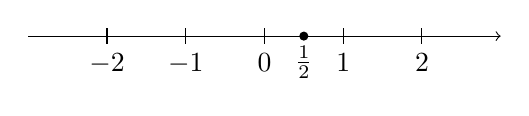
\begin{tikzpicture} 
      \draw[->] (-3,0)--(3,0); 
      % routine for ticks
      \draw (-2,+0.1) -- (-2,-0.1) node[below] {$-2$};
      \draw (-1,+0.1) -- (-1,-0.1) node[below] {$-1$};
      \draw (0,+0.1) -- (0,-0.1) node[below] {$0$};
      \draw (1,+0.1) -- (1,-0.1) node[below] {$1$};
      \draw (2,+0.1) -- (2,-0.1) node[below] {$2$};
      \draw[fill=black] (0.5,0) circle(0.05cm) node[below] {$\frac{1}{2}$};
    \end{tikzpicture}
  \item To represent infinite decimal expansions, we use reasonable
    approximations, e.g., $2.71$ for $e$.
    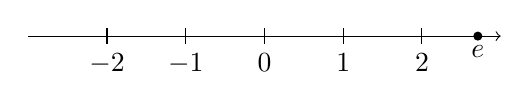
\begin{tikzpicture} 
      \draw[->] (-3,0)--(3,0); 
      % routine for ticks
      \draw (-2,+0.1) -- (-2,-0.1) node[below] {$-2$};
      \draw (-1,+0.1) -- (-1,-0.1) node[below] {$-1$};
      \draw (0,+0.1) -- (0,-0.1) node[below] {$0$};
      \draw (1,+0.1) -- (1,-0.1) node[below] {$1$};
      \draw (2,+0.1) -- (2,-0.1) node[below] {$2$};
      \draw[fill=black] (2.71,0) circle(0.05cm) node[below] {$e$};
    \end{tikzpicture}
  \end{itemize}
\end{frame}

\begin{frame}
  \frametitle{Set Notation}
  \begin{itemize}[<+->]
  \item Another way of representing collections of real numbers is using
    \textit{set builder} notation.
  \item The simplest way to use set notation is just to list the elements
    of the set in curly braces, e.g., $\{ 1, -2, \pi, 1.5 \}$.
  \item We can also put conditions inside the braces: \\
    $\{ x | 0<x<5 \mbox{\ and $x$ is an integer} \}$
  \item That set can also be written $\{1, 2, 3, 4\}$
  \item We read that notation as ``the set of $x$ \textit{such that} $0$
    is less than $x$ which is less than $5$ and $x$ is an integer''.
  \item A wide variety of different conditions can go after the $|$ ``such 
    that'' bar.
  \end{itemize}
\end{frame}

% EJD: integrate pictures of intervals better
\begin{frame}
  \frametitle{Intervals}
  \begin{itemize}[<+->]
  \item Some sets known as \textit{intervals} are so commonly used 
    that we have special notation for them.
  \item An example of an interval is the set $[0,2]=\{x|0\le x \le 2\}$\\
    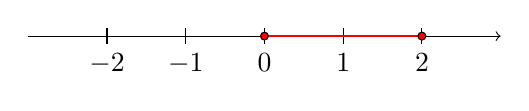
\begin{tikzpicture} 
      \draw[->] (-3,0)--(3,0); 
      % routine for ticks
      \draw (-2,+0.1) -- (-2,-0.1) node[below] {$-2$};
      \draw (-1,+0.1) -- (-1,-0.1) node[below] {$-1$};
      \draw (0,+0.1) -- (0,-0.1) node[below] {$0$};
      \draw (1,+0.1) -- (1,-0.1) node[below] {$1$};
      \draw (2,+0.1) -- (2,-0.1) node[below] {$2$};
      \draw[thick,color=red] (0,0)--(2,0) ;
      \draw[fill=red] (0,0) circle(0.05cm) ;
      \draw[fill=red] (2,0) circle(0.05cm) ;
    \end{tikzpicture}
  \item Another different interval is $(0,2)=\{x|0<x<2\}$\\
    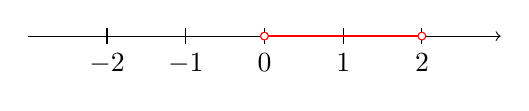
\begin{tikzpicture} 
      \draw[->] (-3,0)--(3,0); 
      % routine for ticks
      \draw (-2,+0.1) -- (-2,-0.1) node[below] {$-2$};
      \draw (-1,+0.1) -- (-1,-0.1) node[below] {$-1$};
      \draw (0,+0.1) -- (0,-0.1) node[below] {$0$};
      \draw (1,+0.1) -- (1,-0.1) node[below] {$1$};
      \draw (2,+0.1) -- (2,-0.1) node[below] {$2$};
      \draw[thick,color=red] (0,0)--(2,0) ;
      \draw[color=red,fill=white] (0,0) circle(0.05cm) ;
      \draw[color=red,fill=white] (2,0) circle(0.05cm) ;
    \end{tikzpicture}
  \item Note the subtle difference between the two examples.
  \item The top interval is \textit{closed}; it includes its endpoints.
  \item The bottom interval is \textit{open}; it does not include
    its endpoints.
  \end{itemize}
\end{frame}

% EJD: graphics!
\begin{frame}
  \frametitle{Table of Intervals}
  \begin{itemize}[<+->]
  %\item We can also have intervals that are open on one end and closed on
  %  another.
  \item Here is a table of all possibilities:
    \begin{tabular}{|c|l|l|}
      \hline
      $[a,b]$            & $\{x|a\le x \le b\}$      & closed             \\
      \hline
      $(a,b)$            & $\{x|a\lt x \lt b\}$      & open               \\
      \hline
      $[a,b)$            & $\{x|a\le x \lt b\}$      & closed-open        \\
      \hline
      $(a,b]$            & $\{x|a\lt x \le b\}$      & open-closed        \\
      \hline
      $[a,\infty)$       & $\{x|a\le x      \}$      & closed-infinite    \\
      \hline
      $(a,\infty)$       & $\{x|a\lt x      \}$      & open-infinite      \\
      \hline
      $(-\infty,b]$      & $\{x|     x \le b\}$      & infinite-closed    \\
      \hline
      $(-\infty,b)$      & $\{x|     x \lt b\}$      & infinite-open      \\
      \hline
      $(-\infty,\infty)$ & $\{x| x\in{\mathbb R} \}$ & infinite-infinite  \\
      \hline
    \end{tabular}
  \item In the above, $\infty$ is \textit{not a number} but is just a notation
    for writing an unbounded interval.
  \end{itemize}
\end{frame}

\subsection{Inequalities}

% EJD: pictures!
\begin{frame}
  \frametitle{Rules for Inequalities}
  \begin{itemize}[<+->]
  \item Often we have to deal with more complicated inequalities.
  \item We need rules to manipulate inequalities correctly.
  \item If $a<b$ then $a+c<b+c$ (add the same number to both sides)
  \item If $a<b$ and $c<d$ then $a+c<b+d$ (add two inequalities)
  \item If $a<b$ and $c>0$ then $ac<bc$ (multiply by a \textit{positive} number)
  \item If $a<b$ and $c<0$ then $ac>bc$ (multiply by a \textit{negative}
    number and \textit{reverse the direction of the inequality}
  \item If $0<a<b$ then $1/a > 1/b$ (in an inequality of positive numbers,
    take reciprocals and \textit{reverse the direction of the inequality}
  \end{itemize}
\end{frame}

% EJD: highlight in red?
% EJD: diagrams?
\begin{frame}
  \frametitle{Multiplying Inequalities by Negatives}
  \begin{itemize}[<+->]
  \item When we work with equalities, we always get equalities when we perform
    correct algebraic manipulations.
  \item However, when we work with inequalities, we sometimes must 
    \textit{reverse} the sign of the inequality.
  \item For example, consider the inequality $1<2$.
  \item Multiplying it by $-1$ we get $-1<-2$ which is incorrect!
  \item When we multiply an inequality by a negative number we must reverse
    the inequality: $1<2 \implies -1>-2$.
  \item We have to be especially careful when we multiply an inequality by
    a variable like $x$: $1<2 \implies x<2x$ \textit{only if we know that
    $x$ is positive}.
  \item If $x=0$ then $x=2x$.
  \item If $x<0$ then $x>2x$.
  \end{itemize}
\end{frame}

% EJD: display equations
\begin{frame}
  \frametitle{Solving Linear Inequalities}
  \begin{itemize}[<+->]
  \item If we solve inequalities, we must be careful if we multiply or divide
    by a number that is negative ($-3$, say) or that \textit{could be negative}
    (the variable $a$, say).
  \item Keeping that in mind, we solve a linear inequality similar to how we
    solve a linear equality.
  \item Consider $x+1 < 3x+5$.
  \item Move all $x$'s to one side, all constants to the other:
    $-2x < 4$
  \item Divide by the (negative!) coefficient of $x$: $x>-2$.
  \item Express the solution set as an interval if you like: 
    $\{x|-2<x\}=(-2,\infty)$
  \end{itemize}
\end{frame}

\begin{frame}
  \frametitle{Solving Multiple Inequalities}
  \begin{itemize}[<+->]
  \item Sometimes we need to solve inequalities like $11\ge 2-3x>5$
  \item In that case, we break it into two separate problems and
    recombine at the end.
  \item $11\ge 2-3x \implies 9\ge -3x \implies -3 \le x$
  \item $2-3x > 5 \implies -3x > 3 \implies x < -1$
  \item Altogether the solution set is $\{x|-3\le x < -1\} = [-3,-1)$
  \item Note that the ``sub-goal'' in each ``sub-problem'' was to 
    \textit{isolate the variable $x$}.
  \item That makes it possible to recombine the sub-results.
  \item Sometimes when we recombine the sub-results, we find that some
    of them are \textit{redundant} in which case they can be dropped.
  \item Sometimes when we recombine the sub-results, we find that some
    of them are \textit{contradictory} in which case the solution set
    is the \textit{empty set} $\varnothing$.
  \end{itemize}
\end{frame}

%% % EJD: save this for when we do graphing
%% \begin{frame}
%%   \frametitle{Using Graphs to Solve Inequalities}
%%   \begin{itemize}[<+->]
%%   \item X
%%   \end{itemize}
%% \end{frame}

\begin{frame}
  \frametitle{Solving Inequalities Involving Quadratics}
  \begin{itemize}[<+->]
  \item Solving inequalities involving quadratics can be difficult.
  \item Consider for example $x^2-4x+3<0$.
  \item Factoring, we have $(x-1)(x-3)<0$.
  \item If we divide by $x-1$ we have to be careful about the cases
    $x-1=0$ and $x-1<0$.
  \item Similarly, if we divide by $x-3$, we have to be careful about
    the cases $x-3=0$ and $x-3<0$.
  \item In general, it is best to avoid dividing by an expression containing
    a variable.
  \item It is best to find another approach.  We will talk about a graphical
    approach later.  Now we will consider using tables.
  \end{itemize}
\end{frame}

% EJD: somehow indicate relations between columns
\begin{frame}
  \frametitle{Using Tables to Solve Inequalities}
  \begin{itemize}[<+->]
  \item Suppose we want to solve $(x-1)(x-3)<0$.
  \item We look for places where the sign of the expression $(x-1)(x-3)$
    changes.
  \item It changes at $x=1$ and $x=3$, so we make up the following table.
    \begin{tabular}{|ccccc|c|c|c|}
      \hline
      \multicolumn{5}{|c|}{$I$} & $(x-1)$  & $(x-3)$        & $(x-1)(x-3)$   \\
      \hline\hline
      $x$&$<$&$1$&$ $&$ $ & \only<4->{$-$} & \only<5->{$-$} & \only<6->{$+$} \\
      \hline
      $x$&$=$&$1$&$ $&$ $ & \only<4->{$0$} & \only<5->{$-$} & \only<6->{$0$} \\
      \hline
      $1$&$<$&$x$&$<$&$3$ & \only<4->{$+$} & \only<5->{$-$} & \only<6->{$-$} \\
      \hline
      $ $&$ $&$x$&$=$&$3$ & \only<4->{$+$} & \only<5->{$0$} & \only<6->{$0$} \\
      \hline
      $ $&$ $&$3$&$<$&$x$ & \only<4->{$+$} & \only<5->{$+$} & \only<6->{$+$} \\
      \hline
    \end{tabular}
  \item<7-> Now we can easily see that the only interval on which $(x-1)(x-3)$
    is negative is $1<x<3$.
  \item<8-> Therefore the solution set to the inequality $(x-1)(x-3)<0$ is
    $\{x|1<x<3\}=(1,3)$.
  \end{itemize}
\end{frame}

\subsection{Absolute Value}

% EJD: picture of absolute value on number line
% EJD: highlight parts of cases construction as 
\begin{frame}
  \frametitle{Definition of Absolute Value}
  \begin{itemize}[<+->]
  \item The absolute value of a number is the magnitude of the number,
    ignoring its sign.
  \item The absolute value of $x$ is written $|x|$.
  \item For example, $|5|=5$, $|-2|=2$, $|\pi|=\pi$, etc.
  \item Formally we define it using \textit{cases}, as follows:
    \begin{equation*}
      |x| = \begin{cases}
         x & \mbox{if $x\ge 0$} \\
        -x & \mbox{if $x<0$}
      \end{cases}
    \end{equation*}
  \item We read that cases construction from the right to the left.
    First we decide which condition the $x$ we are looking at
    satisfies, whether $x\ge 0$ or $x<0$.  Then we look to the left of
    the ``if'' clause to decide which value we take for $|x|$.
  \end{itemize}
\end{frame}

%% \begin{frame}
%%   \frametitle{Cases Notation}
%%   \begin{itemize}[<+->]
%%   \item X
%%   \end{itemize}
%% \end{frame}

% EJD: how do we illustrate this?
\begin{frame}
  \frametitle{Algebraic Properties of Absolute Value}
  \begin{itemize}[<+->]
  \item There is another way to define the absolute value:
    \begin{equation*}
      |x| = \sqrt{x^2}
    \end{equation*}
  \item Think about what happens in that expression when $x\ge 0$ and
    when $x<0$.
  \item It follows by the laws of exponents that the absolute value
    behaves ``nicely'' with respect to multiplication.
  \item We have 
    \begin{equation*}
      |ab| = |a| \, |b| 
      \qquad \left|\frac{a}{b}\right| = \frac{|a|}{|b|}
      \qquad |a^n| = |a|^n
    \end{equation*}
  \end{itemize}
\end{frame}

% EJD: diagram of some kind?
\begin{frame}
  \frametitle{Inequalities and Absolute Value}
  \begin{itemize}[<+->]
  \item Often we use absolute values in conjunction with inequalities.
  \item For example, we might see an expression of the form $|x|<2$.
  \item That means $x$ is less than $2$ in magnitude.
  \item That means $-2<x<2$.  So we have translated $|x|<2$ into an
    inequality without the absolute value sign.
  \item In summary,
    \begin{align*}
      % EJD: do we want to use -a<x<a or (-a<x AND x<a)?
      |x|<a &\Leftrightarrow \mbox{$-a<x$ and $x<a$} \\
      |x|=a &\Leftrightarrow \mbox{$x=-a$ or  $x=a$} \\
      |x|>a &\Leftrightarrow \mbox{$x<-a$ or  $a<x$}
    \end{align*}
  \end{itemize}
\end{frame}

\begin{frame}
  \frametitle{Solving Absolute Value Equations}
  \begin{itemize}[<+->]
  \item Often we have to solve more complicated equations involving
    absolute values.
  \item For example, consider the equation $|2x+1|=5$.
  \item We use the equivalence on the previous slide to rewrite the
    equation as
    \begin{equation*}
      \mbox{$2x+1=-5$ or $2x+1=5$}
    \end{equation*}
  \item We solve each of those equalities separately.  $2x+1=-5$
    implies $2x=-6$ implies $x=-3$.
  \item Similarly, $2x+1=5$ implies $2x=4$ implies $x=2$.
  \item Therefore the solution set is $\{-3,2\}$.
  \item Check by substituting both those numbers into the original
    equation $|2x+1|=5$.
  \end{itemize}
\end{frame}

\begin{frame}
  \frametitle{Solving Absolute Value Inequalities}
  \begin{itemize}[<+->]
  \item Similarly, we often have to solve more complicated inequalities
    involving absolute values.
  \item For example, consider the inequality $|2x+1|<5$.
  \item Using the equivalences on a previous slide, we can translate
    that into an expression that does not involve absolute values
  \item Namely, we have
    \begin{equation*}
      \mbox{$-5<2x+1$ and $2x+1<5$}
    \end{equation*}
  \item Solving the first inequality gives $-6<2x$ or $-3<x$
  \item Solving the second inequality gives $2x<4$ or $x<2$
  \item The condition that $x$ must satisfy is ``$-3<x$ and $x<2$''
  \item We can write it as a single inequality: $-3<x<2$
  \end{itemize}
\end{frame}

% EJD: Illustration of the triangle inequality
\begin{frame}
  \frametitle{The Triangle Inequality}
  \begin{itemize}[<+->]
  \item We will need one more general result about absolute values.
  \item The \textit{triangle inequality} says that the absolute value
    of a sum is less than or equal to the sum of the absolute values.
    \begin{equation*}
      |x+y| \le |x| + |y|
    \end{equation*}
  \item If $x$ and $y$ both have the same sign, the two sides are
    equal.  (Try some examples.)
  \item If $x$ and $y$ have opposite signs, $|x+y|$ is less than
    $|x|+|y|$ because $x$ cancels off part of $y$ in $x+y$.
  \item It's called the \textit{triangle} inequality because the
    numbers $0$, $x$, and $y$ make a (rather flat) triangle in the
    number line.  If $x$ and $y$ have the same sign:
    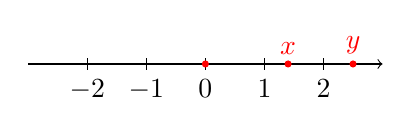
\begin{tikzpicture}[scale=0.75]
      \draw[->] (-3,0)--(3,0); 
      % routine for ticks
      \draw (-2,+0.1) -- (-2,-0.1) node[below] {$-2$};
      \draw (-1,+0.1) -- (-1,-0.1) node[below] {$-1$};
      \draw (0,+0.1) -- (0,-0.1) node[below] {$0$};
      \draw (1,+0.1) -- (1,-0.1) node[below] {$1$};
      \draw (2,+0.1) -- (2,-0.1) node[below] {$2$};
      %\draw[thick,color=red] (0,0)--(2,0) ;
      \draw[color=red,fill=red] (0,0) circle(0.05cm) ;
      \draw[color=red,fill=red] (1.4,0) circle(0.05cm) node[above] {$x$};
      \draw[color=red,fill=red] (2.5,0) circle(0.05cm) node[above] {$y$};
    \end{tikzpicture}
  \item If $x$ and $y$ have opposite signs:
    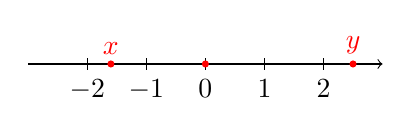
\begin{tikzpicture} [scale=0.75]
      \draw[->] (-3,0)--(3,0); 
      % routine for ticks
      \draw (-2,+0.1) -- (-2,-0.1) node[below] {$-2$};
      \draw (-1,+0.1) -- (-1,-0.1) node[below] {$-1$};
      \draw (0,+0.1) -- (0,-0.1) node[below] {$0$};
      \draw (1,+0.1) -- (1,-0.1) node[below] {$1$};
      \draw (2,+0.1) -- (2,-0.1) node[below] {$2$};
      %\draw[thick,color=red] (0,0)--(2,0) ;
      \draw[color=red,fill=red] (-1.6,0) circle(0.05cm) node[above] {$x$};
      \draw[color=red,fill=red] (0,0)    circle(0.05cm) ;
      \draw[color=red,fill=red] (2.5,0)  circle(0.05cm) node[above] {$y$};
    \end{tikzpicture}
  \end{itemize}
\end{frame}

\end{document}

